% !TEX root = report.tex

% This chapter evaluates LiteCast against state-of-the-art carbon-intensity forecasters across $48$ worldwide regions and a range of workload lengths and slacks.
% The central question is whether the concordance hypothesis of Chapter~3 holds in practice: a lightweight forecaster that optimizes for ordering preservation should match or exceed accuracy-focused models on the realized carbon savings of carbon-aware scheduling.
% We first describe the experimental setup (\S\ref{sec:eval-setup}), then evaluate LiteCast as a standalone forecaster (\S\ref{sec:eval-forecast-quality}) and as the front-end of temporal (\S\ref{sec:eval-temporal}) and spatial (\S\ref{sec:eval-spatial}) carbon-aware schedulers.
% A cluster-trace replay (\S\ref{sec:eval-cluster}) tests practicality on a realistic workload mix, and a closing discussion (\S\ref{sec:eval-discussion}) revisits the design tradeoffs surfaced by the results.

\section{Setup and Methodology}
\label{sec:eval-setup}

% \subsection{Research Questions}
% \label{sec:eval-research-questions}

% The evaluation is organized around two questions.
% \textit{(Q1) Does LiteCast's forecast preserve the ordering of the realized signal across grids of varying renewable penetration?}
% This is the standalone-forecaster question and is answered in \S\ref{sec:eval-forecast-quality}, where we compare LiteCast against CarbonCast on both pointwise accuracy (MAPE) and rank-agreement (concordance).
% \textit{(Q2) Does higher concordance translate into better scheduling outcomes under both temporal and spatial flexibility?}
% This is the question that connects forecast quality to the downstream optimization the forecast feeds, and is answered in \S\ref{sec:eval-temporal} and \S\ref{sec:eval-spatial}.
% \textit{(Q3) Does the adaptive heuristic of \S\ref{sec:method-heuristic} recover additional savings when grid conditions deviate from the training window?}
% This isolates the contribution of the heuristic from the SARIMAX core and is answered alongside Q2 in \S\ref{sec:eval-temporal} and in the cluster-trace replay of \S\ref{sec:eval-cluster}.

\subsection{Energy and Weather Traces}
\label{sec:eval-data}

To train LiteCast, we used publicly available 2023 energy-mix traces and weather data for $48$ regions across the USA and Europe.
US balancing-authority traces are drawn from the EIA's hourly electric-power monitor \cite{eia_data}, European transmission-system-operator traces from the ENTSO-E Transparency Platform \cite{entsoe_data}, and weather observations from the NSF NCAR Research Data Archive for Atmospheric and Ocean Sciences.
Each regional trace reports the hourly breakdown of generation by source (e.g., coal, natural gas, solar, wind, hydro, nuclear), the total electricity demand in $\text{kWh}$, and weather variables including temperature, humidity, wind speed, and solar irradiance.
Electricity demand is used as an exogenous regressor in every region.
The regions used in our experiments span the full carbon-intensity spectrum introduced in Background~\S2.1.4: from low-intensity, low-variability grids dominated by nuclear and hydro (e.g., France, Sweden, Slovakia) to high-intensity, low-variability grids dominated by coal (e.g., Poland, Serbia, Arizona Public Service), and including the high-variability renewable-rich grids that are the central interest of this work (e.g., ERCOT, Denmark, Germany, Lithuania).
The complete list of regions, along with their identifying balancing-authority or TSO code, mean carbon intensity, coefficient of variation, dominant generation source, and aggregate renewable share, is given in Table~\ref{tab:eval-regions}.

Carbon intensity is computed as the demand-weighted average of source-level intensities using the IPCC AR5 operational carbon factors \cite{ipcc_carbon_factors_2014} introduced in Background~\S2.1.2, expressed in $\text{g}\cdot\text{CO}_2\text{eq}/\text{kWh}$ at hourly granularity.
Hourly granularity is the highest resolution at which average carbon intensity is publicly reported across this set of regions, and the grid's intensity rarely varies meaningfully on sub-hourly timescales, so finer resolution would not materially change the results.
The evaluation uses 2023 for both training and testing of LiteCast (which trains on a month-long rolling window ending at each job's submission time, see \S\ref{sec:eval-implementation}); CarbonCast, which requires a longer training history, uses all of 2022 to forecast over 2023.

{\footnotesize
\setlength{\tabcolsep}{4pt}
\renewcommand{\arraystretch}{1.0}
\begin{longtable}{@{}llrrlr@{}}
\caption{The $48$ regions used in the evaluation, sorted by mean carbon intensity. Mean CI is in $\text{g}\cdot\text{CO}_2\text{eq}/\text{kWh}$. CV is the coefficient of variation ($\sigma/\mu$) over 2023. Dominant source lists the largest share of generation; renewable share aggregates wind, solar, and hydro.}
\label{tab:eval-regions} \\
\toprule
Region & Code & Mean CI & CV & Dominant source & Renew.\ (\%) \\
\midrule
\endfirsthead
\multicolumn{6}{c}{\tablename\ \thetable{} -- continued from previous page} \\
\toprule
Region & Code & Mean CI & CV & Dominant source & Renew.\ (\%) \\
\midrule
\endhead
\midrule
\multicolumn{6}{r}{continued on next page} \\
\endfoot
\bottomrule
\endlastfoot
Switzerland & CH & 0 & --- & nuclear (57\%) & 43 \\
France & FR & 24 & 0.65 & nuclear (67\%) & 25 \\
PacifiCorp West & PACW & 43 & 0.69 & hydro (44\%) & 94 \\
Bonneville Power Administration & BPAT & 44 & 0.39 & hydro (71\%) & 79 \\
Austria & AT & 46 & 1.00 & hydro (64\%) & 84 \\
Finland & FI & 54 & 0.77 & nuclear (47\%) & 39 \\
Lithuania & LT & 67 & 0.95 & wind (47\%) & 69 \\
Southwestern Power Administration & SPA & 82 & 1.75 & hydro (86\%) & 86 \\
Slovakia & SK & 86 & 0.25 & nuclear (63\%) & 17 \\
Idaho Power & IPCO & 100 & 0.54 & hydro (55\%) & 76 \\
Spain & ES & 102 & 0.45 & wind (25\%) & 51 \\
Portugal & PT & 104 & 0.67 & wind (33\%) & 66 \\
Sweden & SE & 117 & 0.19 & nuclear (43\%) & 26 \\
Belgium & BE & 120 & 0.36 & nuclear (39\%) & 29 \\
Denmark & DK & 122 & 0.69 & wind (58\%) & 68 \\
Latvia & LV & 127 & 0.79 & hydro (64\%) & 68 \\
Texas & ERCO & 130 & 0.27 & wind (46\%) & 55 \\
Hungary & HU & 159 & 0.26 & nuclear (48\%) & 17 \\
Croatia & HR & 165 & 0.35 & hydro (46\%) & 65 \\
Slovenia & SI & 175 & 0.48 & nuclear (38\%) & 37 \\
California ISO & CISO & 185 & 0.36 & natural gas (46\%) & 42 \\
Salt River Project & SRP & 186 & 0.23 & nuclear (52\%) & 4 \\
Duke Energy Carolinas & DUK & 217 & 0.19 & nuclear (54\%) & 6 \\
Tennessee Valley Authority & TVA & 224 & 0.15 & nuclear (44\%) & 11 \\
Greece & GR & 231 & 0.41 & natural gas (38\%) & 52 \\
ISO New England & ISNE & 244 & 0.12 & natural gas (58\%) & 13 \\
Italy & IT & 254 & 0.24 & natural gas (45\%) & 36 \\
Germany & DE & 268 & 0.43 & wind (30\%) & 47 \\
Turlock Irrigation District & TIDC & 272 & 0.20 & natural gas (74\%) & 26 \\
Bulgaria & BG & 273 & 0.28 & nuclear (41\%) & 20 \\
PJM Interconnection & PJM & 280 & 0.09 & natural gas (44\%) & 7 \\
South Carolina E\&G & SCEG & 285 & 0.22 & natural gas (47\%) & 10 \\
Florida Power \& Light & FPL & 302 & 0.10 & natural gas (58\%) & 7 \\
Southwest Power Pool & SWPP & 305 & 0.33 & wind (37\%) & 40 \\
Southern Company & SOCO & 326 & 0.09 & natural gas (54\%) & 7 \\
Czechia & CZ & 326 & 0.19 & nuclear (41\%) & 8 \\
El Paso Electric & EPE & 333 & 0.13 & natural gas (90\%) & 10 \\
Public Service Co.\ of Colorado & PSCO & 343 & 0.25 & wind (31\%) & 40 \\
Nevada Power & NEVP & 347 & 0.23 & natural gas (61\%) & 21 \\
Estonia & EE & 348 & 0.46 & coal (42\%) & 34 \\
LA Dept.\ of Water \& Power & LDWP & 352 & 0.27 & natural gas (46\%) & 28 \\
Midcontinent ISO & MISO & 359 & 0.14 & natural gas (39\%) & 18 \\
Netherlands & NL & 402 & 0.16 & natural gas (39\%) & 16 \\
Arizona Public Service & AZPS & 439 & 0.21 & natural gas (46\%) & 17 \\
PacifiCorp East & PACE & 452 & 0.22 & coal (47\%) & 28 \\
NorthWestern Energy (MT) & NWMT & 470 & 0.17 & coal (60\%) & 35 \\
Serbia & RS & 481 & 0.19 & coal (61\%) & 1 \\
Associated Electric Cooperative & AECI & 502 & 0.12 & coal (46\%) & 12 \\
Poland & PL & 532 & 0.18 & coal (64\%) & 24 \\
South Carolina Public Service & SC & 590 & 0.09 & coal (61\%) & 5 \\
\end{longtable}
}

\subsection{Workload Model}
\label{sec:eval-workload}

Although the design applies to any flexible electrical load, we construct an artificial workload model that exhaustively sweeps across common job lengths and slack lengths to verify that the model is sound across the year for any job it encounters.
Each job draws a unit power of approximately $1\,\text{W}$ and must complete within a window of length $\mathcal{J}_{\text{window}} = \mathcal{J}_{\text{length}} + \mathcal{J}_{\text{slack}}$, following the formalism of \S\ref{sec:method-formulation}.
Job length $\mathcal{J}_{\text{length}}$ is swept over $\{1, 6, 12, 24, 48\}$ hours and slack $\mathcal{J}_{\text{slack}}$ over $\{24, 48, 96, 168\}$ hours, and we evaluate every combination of the two, representing demand ranging from short interactive batch jobs through multi-day AI training workloads with weeklong deadlines.
Because we report carbon optimality as a ratio against the oracle, the choice of unit power does not affect any of the results.
A separate evaluation in \S\ref{sec:eval-cluster} replays a real cluster workload trace to test that the conclusions of the synthetic sweep survive a realistic job-mix distribution.

For each (region, $\mathcal{J}_{\text{length}}$, $\mathcal{J}_{\text{slack}}$) configuration we evaluate two job models from \S\ref{sec:method-formulation}.
\textit{Continuous} jobs must run uninterrupted for $\mathcal{J}_{\text{length}}$ consecutive hours within the window.
\textit{Interruptible} jobs may run on any $\mathcal{J}_{\text{length}}$ hours within the window via checkpoint-restore, choosing the lowest-intensity subset.
The two models bracket the practical flexibility regimes a cluster scheduler encounters: long-running simulations and training jobs that cannot tolerate interruption sit at the continuous extreme, while data-parallel batch workloads and electric car charging sit closer to the interruptible extreme.
For each configuration we schedule jobs across submission dates throughout 2023 and aggregate the realized emissions across regions and submissions.

\subsection{Baselines}
\label{sec:eval-baselines}

We compare LiteCast against three alternative forecasters and against an oracle.

\paragraph{Persistence.}
The naive baseline reuses the previous day's hourly carbon-intensity observations as the prediction for the next day.
It captures the strong diurnal cycle present in most grids but nothing else: weather-driven deviations, weekly cycles, and slow trends are all invisible to it.
Persistence is parameter-free and serves as the floor against which any nontrivial forecaster must improve.

\paragraph{CarbonCast.}
CarbonCast \cite{maji_carboncast_2022} is the state-of-the-art deep-learning forecaster discussed in Background~\S2.3.
It uses a two-tier architecture, with a per-source neural network followed by an aggregation stage that combines per-source forecasts into a regional carbon-intensity forecast.
The published model produces hourly forecasts up to $96$ hours ahead; we extend it to the $168$-hour horizon used here by chaining its own forecasts as inputs, following the procedure in its public repository.
% CarbonCast is trained on all of 2022 to forecast 2023.
CarbonCast requires a year's worth of training data to forecast half a year.
CarbonCast forecasted the first half of 2023 using the entire 2022 data, and the second half of 2023 using the second half of 2022 and the first half of 2023. 
CarbonCast represents the heavyweight, accuracy-focused class of forecasters: it requires substantial historical data, fixed-architecture neural networks, and GPU-class compute to train.

\paragraph{LiteCast.}
% LiteCast denotes the per-source SARIMAX pipeline of \S\ref{sec:method-litecast} without the adaptive heuristic.
LiteCast denotes the per-source SARIMAX pipeline of \S\ref{sec:method-litecast}.
It trains on a month-long rolling window of hourly energy, weather, and demand data ending at the job's submission time, trains a new model on each submission, and produces deterministic forecasts over the requested horizon.

% \paragraph{LiteCast + Heuristic.}
% This configuration adds the adaptive scheduling heuristic of \S\ref{sec:method-heuristic} on top of the LiteCast forecaster.
% The heuristic monitors the forecast used to make a decision against a pseudo-oracle constructed from observations that have arrived since the job was submitted and triggers a re-forecast whenever the running concordance falls below the configured threshold, accepting the new schedule with probability $p_1$ to damp oscillation.
% The configuration isolates the contribution of online adaptation from the underlying SARIMAX forecaster.

\paragraph{Oracle.}
The oracle is a hypothetical scheduler that has perfect knowledge of $f^{\text{act}}$ over the full window and selects the minimum-emissions schedule under Eq.~\ref{eq:method-continuous-start} (continuous) or Eq.~\ref{eq:method-interruptible-set} (interruptible).
The oracle is never available to a forecaster in practice; it serves only as the upper bound against which realized emissions are normalized.
A forecaster with high optimality represents a model that is close to oracle knowledge. 
% Two state-of-the-art forecasters are deliberately not included.
% EnsembleCI \cite{yan_ensembleci_2025} is an ensemble extension of CarbonCast but has no publicly available $168$-hour configuration at the time of writing; commercial APIs such as Electricity Maps and WattTime are not directly reproducible.
% We discuss the implications of these omissions in \S\ref{sec:eval-discussion}.

\subsection{Metrics}
\label{sec:eval-metrics}

We report five metrics across this chapter, grouped into three categories.

\paragraph{Forecast-quality metrics.}
\textit{MAPE} measures the mean absolute percentage error between $\hat{f}$ and $f^{\text{act}}$ over the forecast window.
It is the prevailing optimization target in the carbon-intensity forecasting literature, where lower is better.
\textit{Concordance} $C(\hat{f}, f^{\text{act}})$ is the rank-agreement metric defined in Eq.~\ref{eq:method-concordance}; values near $1$ indicate that the forecast preserves the pairwise ordering of carbon intensities across the window, while $0.5$ is no better than chance.
We include these metrics to show that LiteCast achieves higher concordance than competitor models, while also remaining at least as accurate.
% Together MAPE and $C$ characterize the same forecast along two axes: how close the values are and how well their ordering matches.

\paragraph{Scheduling-outcome metrics.}
\textit{Carbon optimality} is the ratio $\rho = E_{\text{pred}} / E_{\text{oracle}}$ defined in Eq.~\ref{eq:method-rho}, expressed as a percentage of the oracle.
A policy with $\rho = 1$ achieves $100\%$ carbon optimality. 
With $\rho = 1$, the scheduler chose the most optimal decision and cannot do any better.
% We also report \textit{additional emissions}, defined as $(\rho - 1) \cdot 100\%$, which we use in figures where the differences between policies are small and the additional-emissions framing is more legible.
We also report \textit{additional emissions}, defined as $(\rho - 1) \cdot 100\%$, which we use in figures where there are few policies to show and we are comparing to the oracle.
% We also report \textit{carbon savings}, defined as $100 - (\rho - 1) \cdot 100\%$, which we use in figures where the differences between policies are small and the additional-emissions framing is more legible.
% \textit{Region-win rate} is the fraction of (length, slack, date) tuples for which a spatial-flexibility forecaster selects the same execution region as the oracle.
% It is reported only in the spatial-scheduling analysis of \S\ref{sec:eval-spatial}.

\paragraph{Regional-difficulty metric.}
\textit{Coefficient of variation} (CV) is $\sigma / \mu$ of a region's hourly carbon intensity over 2023, with $\sigma$ the standard deviation and $\mu$ the mean.
CV proxies the difficulty of carbon-aware scheduling in a region: a flat-intensity grid (low CV) offers little to optimize against, while a highly variable grid (high CV) offers large potential savings but also large scope for ordering errors.
We use CV as the per-region $x$-axis throughout the chapter when grouping regions by their scheduling difficulty.

\subsection{Implementation and Infrastructure}
\label{sec:eval-implementation}

% LiteCast and its heuristic are implemented in Python~3.10, using the SARIMAX implementation in \texttt{statsmodels} \cite{statsmodels} configured as described in \S\ref{sec:method-model}.
LiteCast is implemented in Python~3.10, using the SARIMAX implementation in \texttt{statsmodels} \cite{statsmodels} configured as described in \S\ref{sec:method-model}.
CarbonCast is reimplemented from its public repository against the same energy, weather, and demand inputs as LiteCast, so any forecast-quality differences between the two reflect modelling choices and not data access.
The contrast in training-data size is substantial: LiteCast trains on a month-long window of hourly observations, while CarbonCast trains on all of 2022, which results in up to a $12\times$ difference.
All forecasts are evaluated against the realized 2023 carbon-intensity trace described in \S\ref{sec:eval-data}.

All experiments are executed on the National Research Platform \cite{weitzel_nrp_2025}, a multi-tenant Kubernetes cluster operated by UC San Diego and partners.
The computation is parallelized across jobs in Nautilus, and forecasts are written to a central PostgreSQL database from which the figures in this chapter are generated.
% The Bernoulli accept step inside the heuristic is seeded so that, given the same trace and configuration, repeated runs are byte-identical; SARIMAX fits in \texttt{statsmodels} are deterministic on a fixed input.

\section{Forecast Quality}
\label{sec:eval-forecast-quality}

We first compare LiteCast and CarbonCast as standalone forecasters along the two axes introduced above, deferring the scheduling-outcome analysis to \S\ref{sec:eval-temporal} and \S\ref{sec:eval-spatial}.
The goal here is to characterize each forecaster's MAPE and concordance independently of any downstream scheduler, so that we can later separate the two questions: \textit{is the forecast concordant?} and \textit{is it useful for scheduling?}

\subsection{Per-Region Forecast Traces}
\label{sec:eval-forecast-traces}

\begin{figure}[!htbp]
    \centering
    \begin{subfigure}[t]{0.48\linewidth}
        \centering
        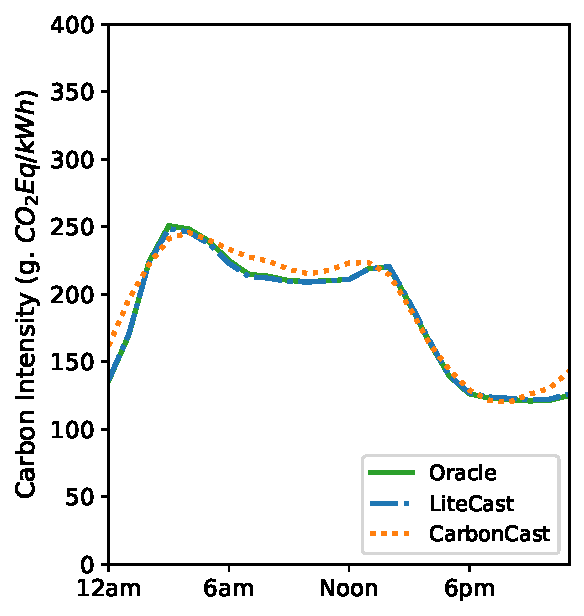
\includegraphics[width=\linewidth]{images/evaluation/ciso_compare.pdf}
        \caption{California (CISO)}
        \label{fig:eval-forecast-ciso}
    \end{subfigure}
    \hfill
    \begin{subfigure}[t]{0.48\linewidth}
        \centering
        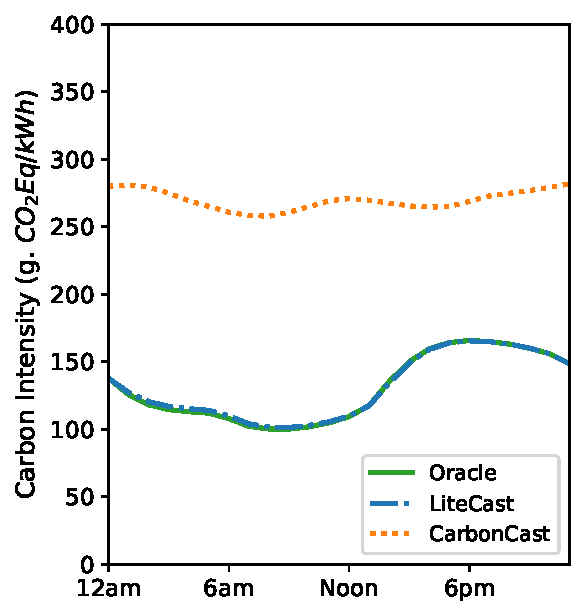
\includegraphics[width=\linewidth]{images/evaluation/erco_compare.pdf}
        \caption{Texas (ERCOT)}
        \label{fig:eval-forecast-erco}
    \end{subfigure}

    \vspace{0.5em}

    \begin{subfigure}[t]{0.48\linewidth}
        \centering
        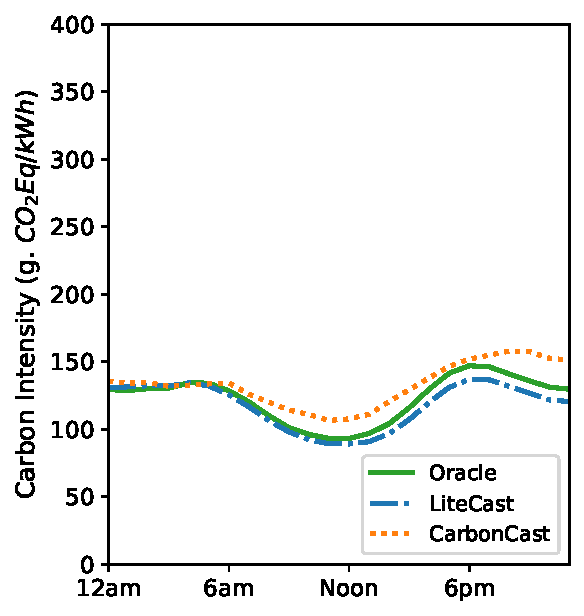
\includegraphics[width=\linewidth]{images/evaluation/dk_compare.pdf}
        \caption{Denmark (DK)}
        \label{fig:eval-forecast-dk}
    \end{subfigure}
    \hfill
    \begin{subfigure}[t]{0.48\linewidth}
        \centering
        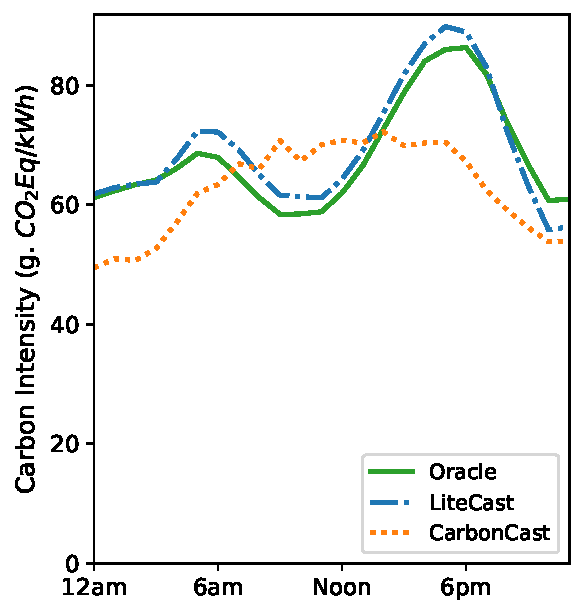
\includegraphics[width=\linewidth]{images/evaluation/LT_compare.pdf}
        \caption{Lithuania (LT)}
        \label{fig:eval-forecast-de}
    \end{subfigure}
    \caption{Average $24$-hour carbon-intensity forecasts for four representative regions in 2023.}
    \label{fig:eval-forecast-timeseries}
\end{figure}

Figure~\ref{fig:eval-forecast-timeseries} shows the average hourly carbon-intensity forecasts for four representative regions over a $24$-hour window in 2023.
The four regions are chosen to span the range of grid characteristics that matter for forecasting.
California (CISO) is moderately renewable-heavy and exhibits a smooth midday solar trough.
Texas (ERCOT) has a wind-dominated mix that produces large overnight troughs but is less regular than California's diurnal pattern.
Denmark (DK) and Lithuania (LT) are wind-rich European grids with the highest hourly variability in our $48$-region set.

LiteCast tracks the oracle's diurnal shape closely in all four regions, including in Denmark and Lithuania where sharp wind-driven swings dominate.
CarbonCast captures the broader trend in California but consistently under- or over-estimates the magnitude of troughs and peaks in Texas and Lithuania.
The pattern reflects a structural mismatch: CarbonCast's training on a full year of 2022 data smooths over the weather shifts that drive Texas's and Lithuania's 2023 carbon intensity, while LiteCast's month-long window keeps it locally calibrated to whichever weather regime is currently in force.

\subsection{MAPE versus Concordance}
\label{sec:eval-mape-vs-concordance}

\begin{figure}[!htbp]
    \centering
    \begin{subfigure}[t]{0.48\linewidth}
        \centering
        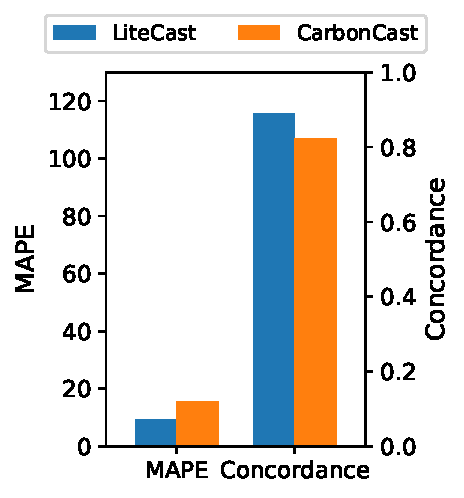
\includegraphics[width=\linewidth]{images/evaluation/CISO_metrics.pdf}
        \caption{California (CISO)}
        \label{fig:eval-metrics-ciso}
    \end{subfigure}
    \hfill
    \begin{subfigure}[t]{0.48\linewidth}
        \centering
        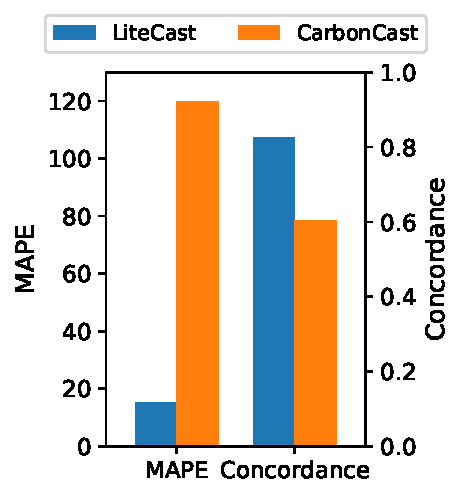
\includegraphics[width=\linewidth]{images/evaluation/ERCO_metrics.pdf}
        \caption{Texas (ERCOT)}
        \label{fig:eval-metrics-erco}
    \end{subfigure}

    \vspace{0.5em}

    \begin{subfigure}[t]{0.48\linewidth}
        \centering
        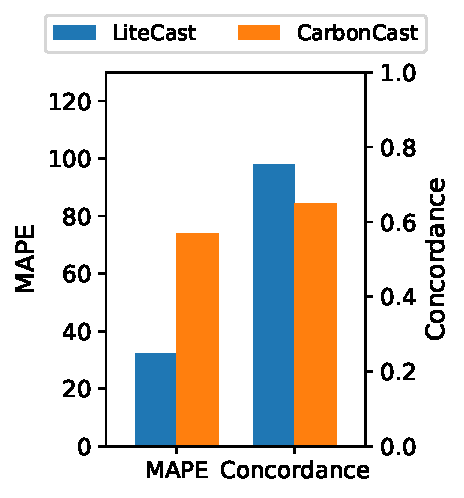
\includegraphics[width=\linewidth]{images/evaluation/DK_metrics.pdf}
        \caption{Denmark (DK)}
        \label{fig:eval-metrics-dk}
    \end{subfigure}
    \hfill
    \begin{subfigure}[t]{0.48\linewidth}
        \centering
        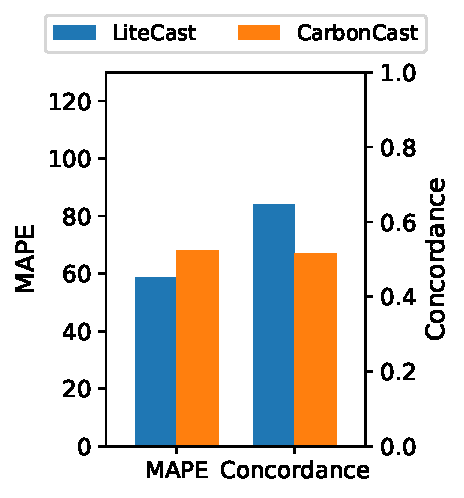
\includegraphics[width=\linewidth]{images/evaluation/LT_metrics.pdf}
        \caption{Lithuania (LT)}
        \label{fig:eval-metrics-lt}
    \end{subfigure}
    \caption{Concordance (higher is better) and MAPE (lower is better) for LiteCast and CarbonCast across four representative regions.}
    \label{fig:eval-mape-vs-concordance}
\end{figure}

Figure~\ref{fig:eval-mape-vs-concordance} compares LiteCast and CarbonCast along both forecast-quality axes across all four regions.
LiteCast outperforms CarbonCast on both metrics in every region: it achieves both a lower MAPE and a higher concordance index in California, Texas, Denmark, and Lithuania.
These plots show that LiteCast achieves higher concordance than a heavyweight model trained over a full year, which is the metric that actually governs scheduling outcomes, and as a secondary observation also achieves lower MAPE.
LiteCast's month-long rolling window keeps it locally calibrated to whichever weather regime is currently driving the grid: when a windy week shifts to a calm one, LiteCast refits on the new conditions within hours.
CarbonCast averages across regime shifts that LiteCast's rolling window resolves, which is why its forecasts in renewable-heavy grids such as Denmark and Lithuania consistently lag the trends in the realized signal.

This result does not weaken the argument of \S\ref{sec:method-concordance} that concordance, not accuracy, is the metric that matters for scheduling.
The two gaps in Figure~\ref{fig:eval-mape-vs-concordance} are not proportional across regions, and \S\ref{sec:eval-temporal-samples} shows that it is concordance, not MAPE, that impacts realized carbon savings.
LiteCast's MAPE advantage is incidental; its concordance advantage is what carries the scheduling results.

\subsection{Takeaway}
\label{sec:eval-forecast-takeaway}

Across these four representative regions, LiteCast dominates CarbonCast on both forecast-quality metrics, with the largest absolute gains in the renewable-heavy grids where adapting to recent regime shifts matters most.
The two metrics do not move in lockstep, however, and the next sections turn from forecast quality to scheduling outcomes to show that it is the concordance gap, not the MAPE gap, that predicts realized carbon savings across the full $48$-region set.

\section{Temporal Carbon-Aware Scheduling}
\label{sec:eval-temporal}

We now plug each forecaster into the temporal scheduler of \S\ref{sec:method-formulation} and measure realized emissions across the full grid of job lengths, slacks, regions, and submission dates.
The temporal scheduler defers a job within a single region; the spatial extension in \S\ref{sec:eval-spatial} adds the choice of execution region.

\subsection{Sample Schedules}
\label{sec:eval-temporal-samples}

\begin{figure}[!htbp]
    \centering
    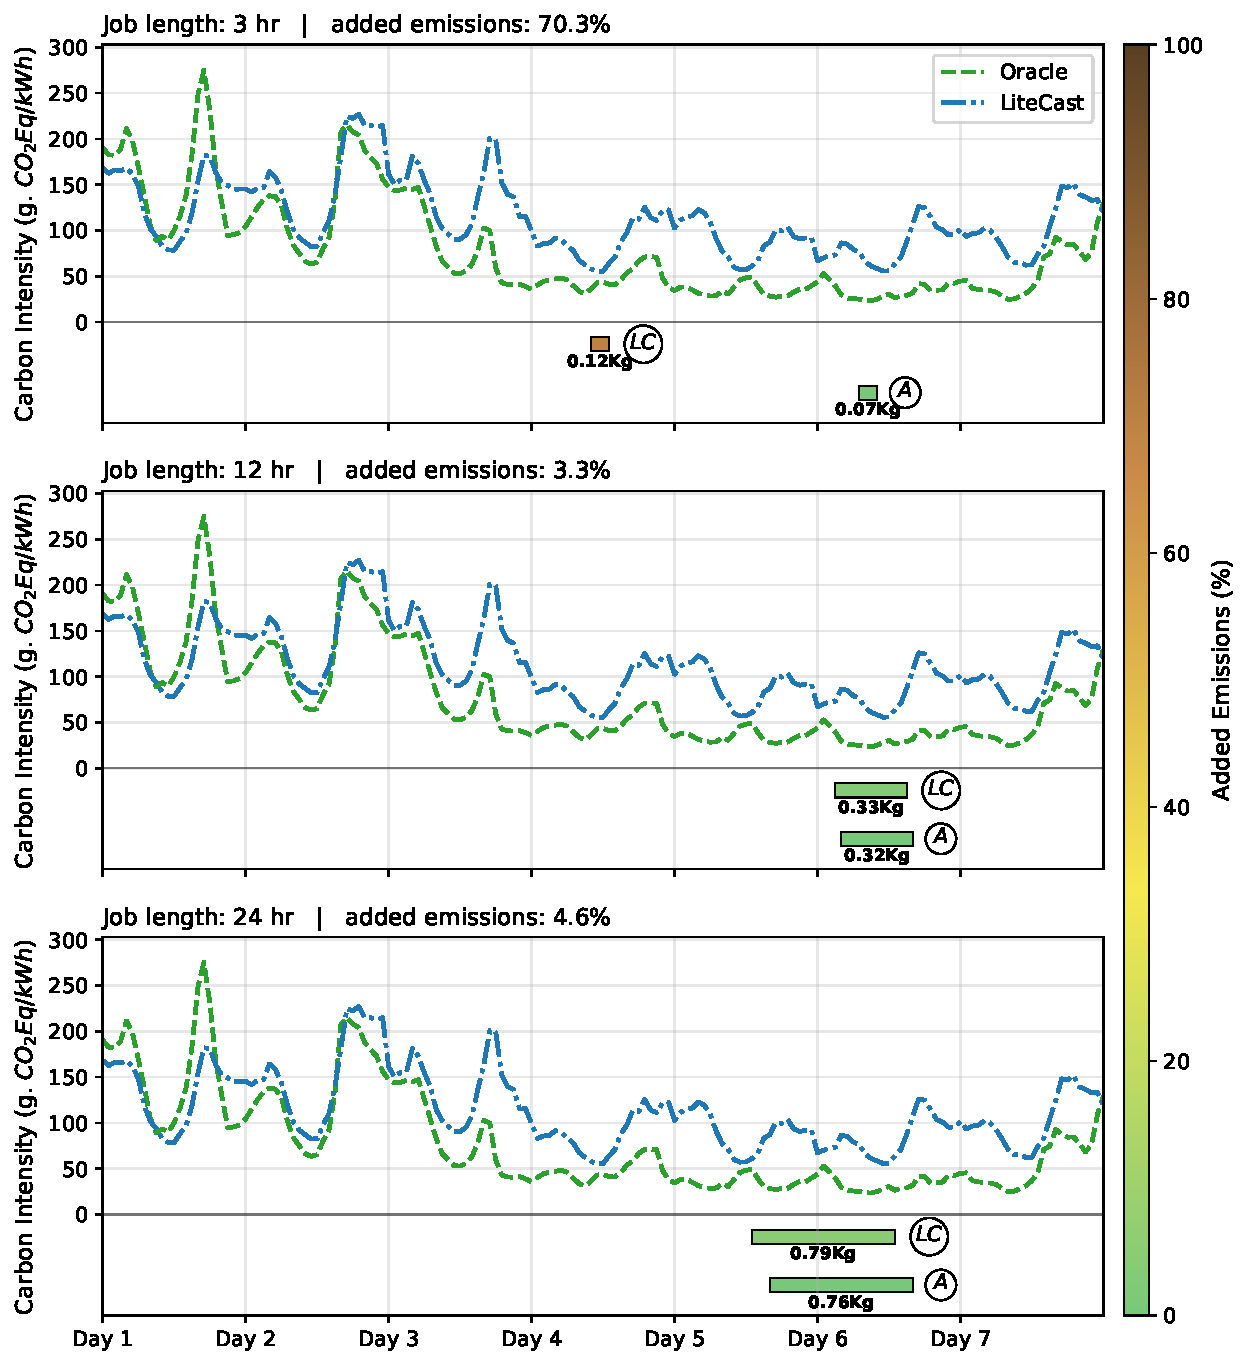
\includegraphics[width=0.95\linewidth]{images/evaluation/DK_scheduling_2023_09_15.pdf}
    \caption{Forecast versus oracle sample schedules over a seven-day window in Denmark, beginning 2023-09-15. Circles labelled $A_i$ mark the oracle's chosen start hour for length $i$; circles labelled $LC_i$ mark LiteCast's start hour.}
    \label{fig:eval-sample-schedules}
\end{figure}

Figure~\ref{fig:eval-sample-schedules} shows a weeklong example of carbon-aware scheduling in Denmark, with three continuous jobs of $3$, $12$, and $24$ hours all submitted on the first day of the window.
For the $12$-hour and $24$-hour jobs, LiteCast's chosen start hour is slightly offset from the oracle's, but both forecaster and oracle land on the same low-emission portion of the week, so the realized emissions of LiteCast's schedules are within a small margin of the oracle's.
This is the concordance argument made concrete: when the forecast preserves the ordering of windowed sums over the slack horizon, the scheduler picks a start hour that is at or near the oracle's optimum, even when the forecasted intensities themselves are not exact.

The $3$-hour job is harder.
Shorter jobs are more sensitive to the within-day ranking of individual hours, because the scheduler is now selecting among many candidate three-hour windows whose total emissions can differ by small amounts that the forecaster must rank correctly.
A forecast with high overall concordance but small local mis-orderings within the day can pick a three-hour window that is several percentage points worse than the oracle's, even when the same forecast schedules the longer jobs optimally.
Concordance gains have larger marginal value as job length shrinks, because shorter jobs leave less room for the scheduling decision to ``land on'' a low-emission region by accident.

\subsection{Continuous Jobs}
\label{sec:eval-temporal-continuous}

\begin{figure}[!htbp]
    \centering
    \begin{subfigure}[t]{0.48\linewidth}
        \centering
        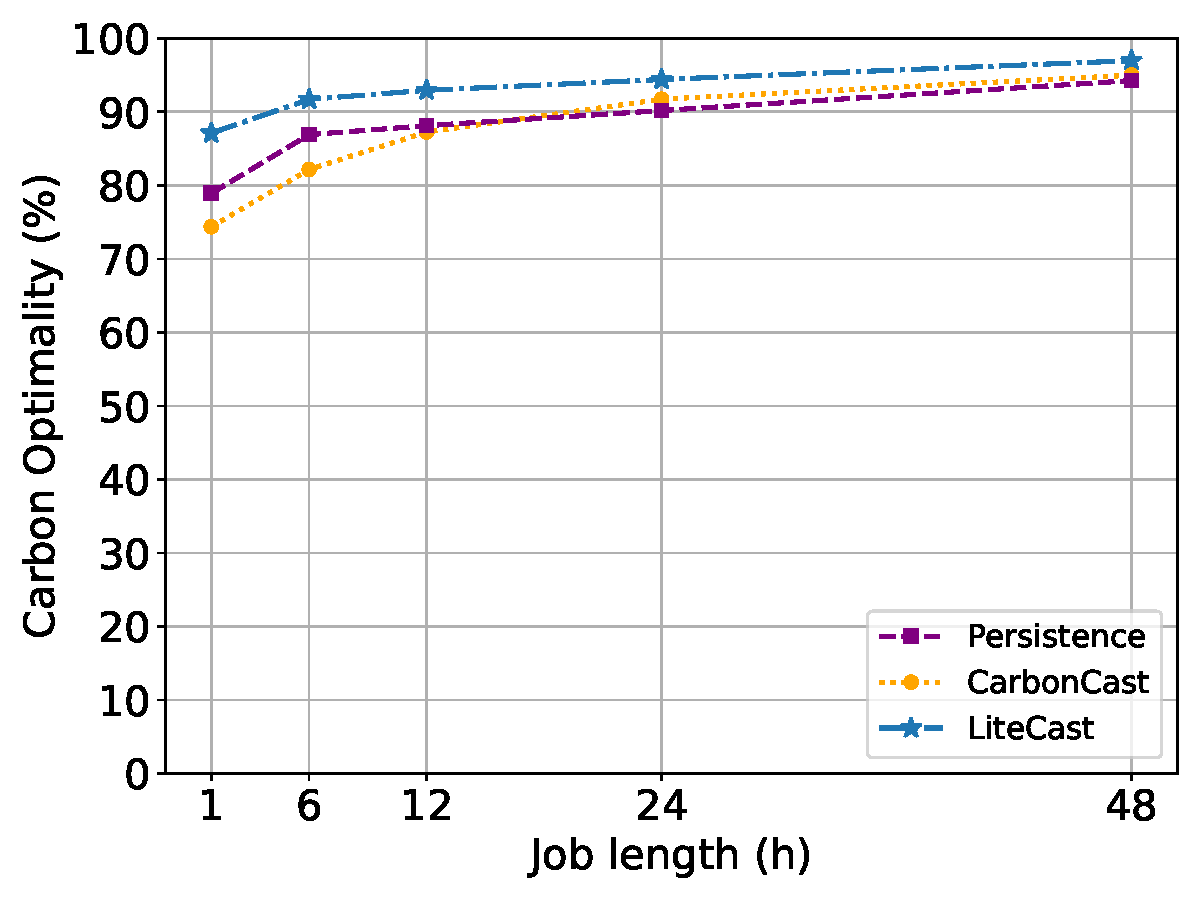
\includegraphics[width=\linewidth]{images/evaluation/fixed_slack/continuous/Continuous_Jobs_with_24_Hour_Slack_ensemble.pdf}
        \caption{$24$-hour slack}
        \label{fig:eval-continuous-24h}
    \end{subfigure}
    \hfill
    \begin{subfigure}[t]{0.48\linewidth}
        \centering
        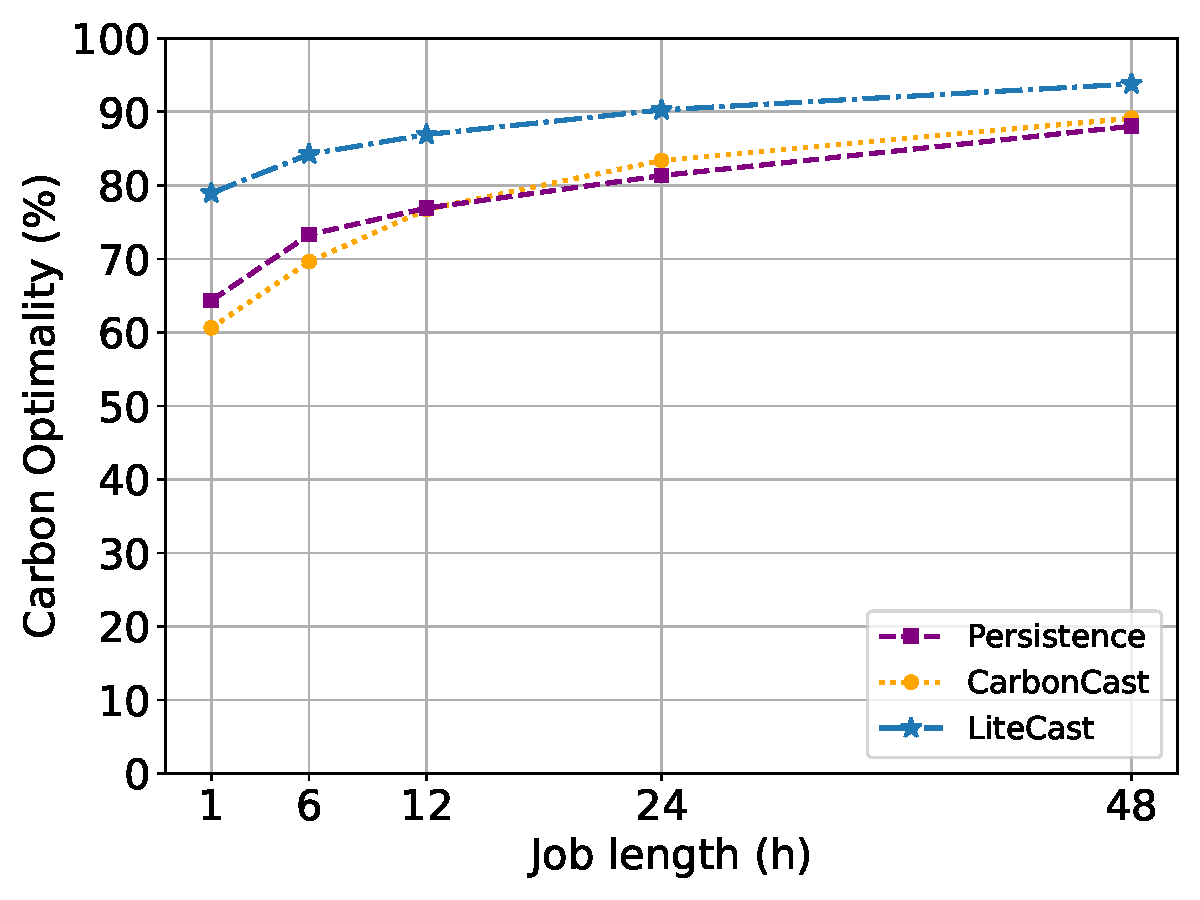
\includegraphics[width=\linewidth]{images/evaluation/fixed_slack/continuous/Continuous_Jobs_with_48_Hour_Slack_ensemble.pdf}
        \caption{$48$-hour slack}
        \label{fig:eval-continuous-48h}
    \end{subfigure}

    \vspace{0.5em}

    \begin{subfigure}[t]{0.48\linewidth}
        \centering
        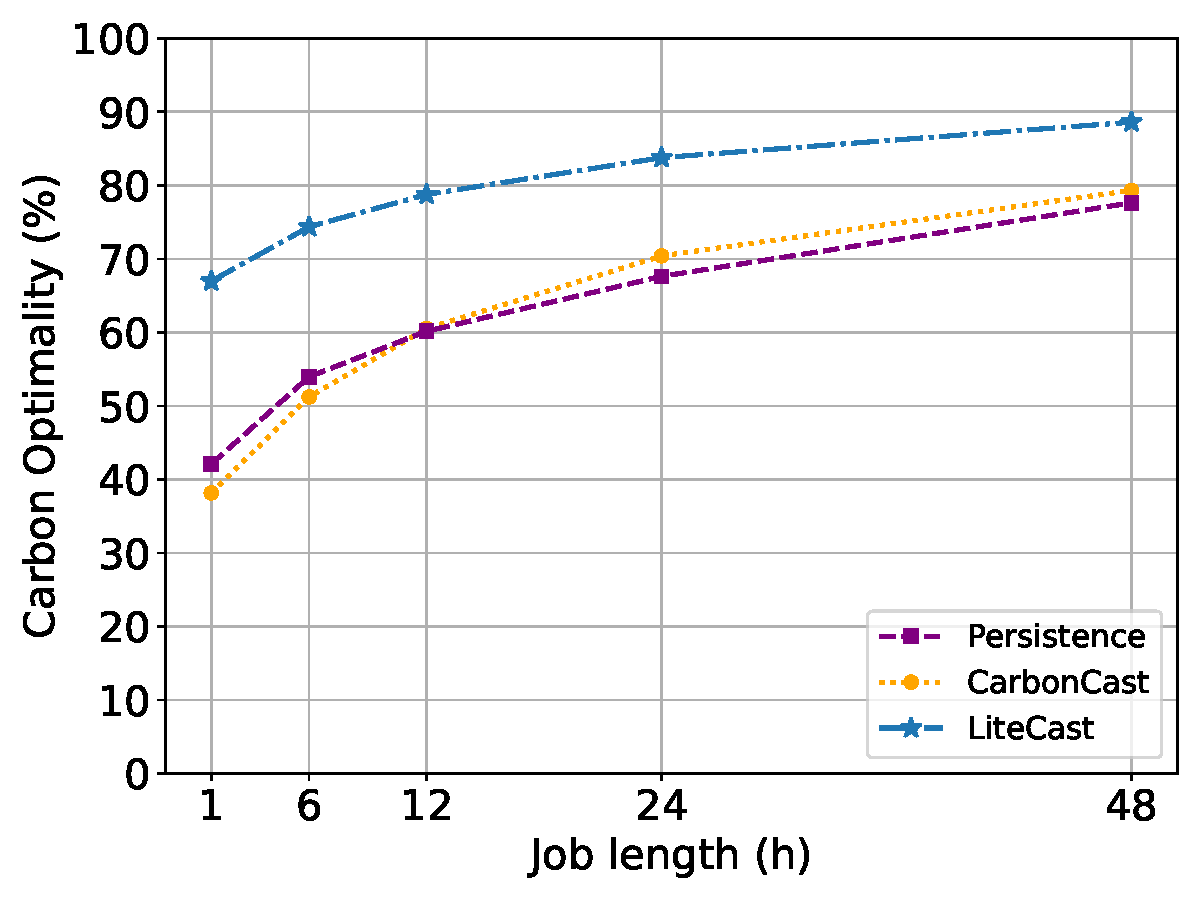
\includegraphics[width=\linewidth]{images/evaluation/fixed_slack/continuous/Continuous_Jobs_with_96_Hour_Slack_ensemble.pdf}
        \caption{$96$-hour slack}
        \label{fig:eval-continuous-96h}
    \end{subfigure}
    \hfill
    \begin{subfigure}[t]{0.48\linewidth}
        \centering
        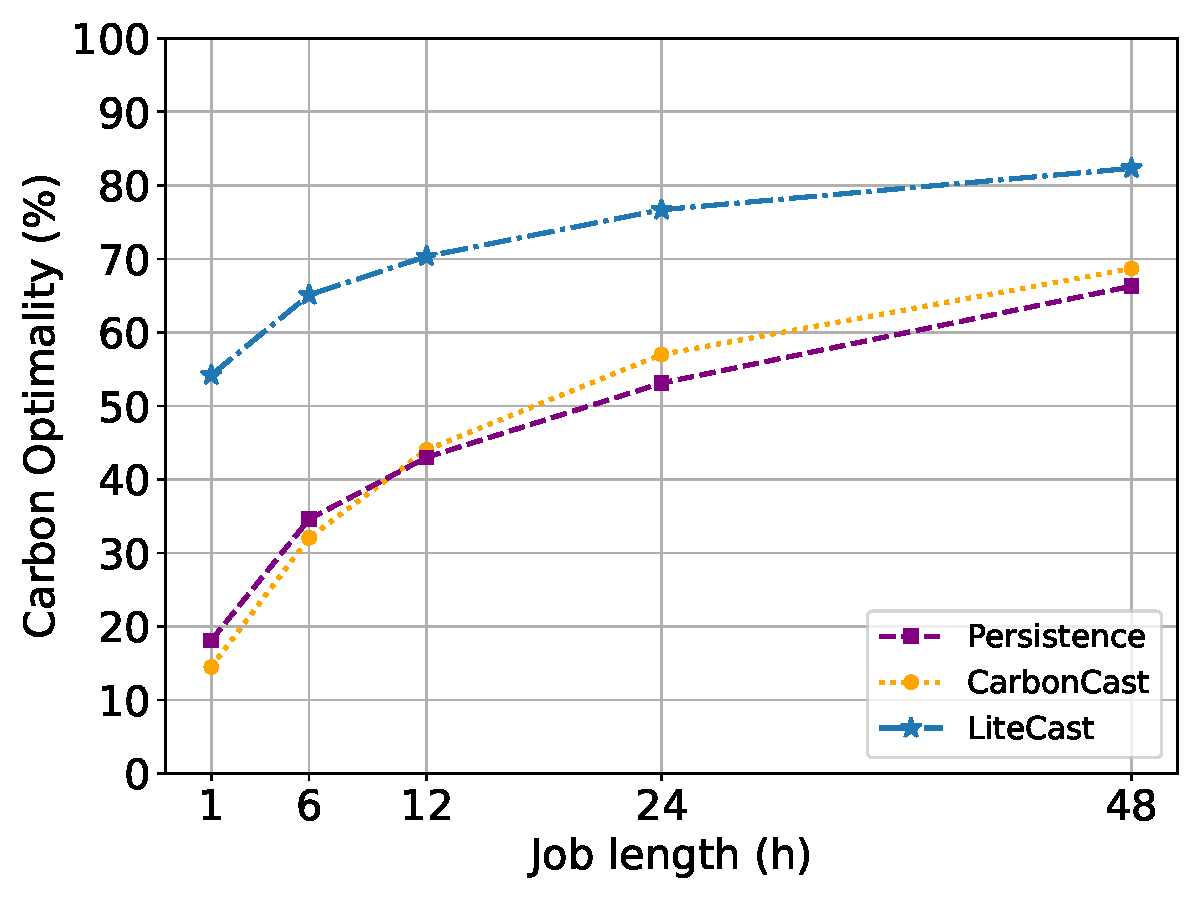
\includegraphics[width=\linewidth]{images/evaluation/fixed_slack/continuous/Continuous_Jobs_with_168_Hour_Slack_ensemble.pdf}
        \caption{$168$-hour slack}
        \label{fig:eval-continuous-168h}
    \end{subfigure}
    \caption{Carbon optimality across all $48$ regions for continuous jobs.}
    \label{fig:eval-carbon-optimality-continuous}
\end{figure}

Figure~\ref{fig:eval-carbon-optimality-continuous} reports average carbon optimality across all $48$ regions for continuous jobs, broken out by slack at $24$, $48$, $96$, and $168$ hours.
Two patterns emerge.
First, LiteCast outperforms CarbonCast at every length-slack configuration, by an average of $5$--$20\%$ depending on the slack.
% Second, LiteCast~+~Heuristic delivers a further improvement, achieving up to $97\%$ carbon optimality for jobs shorter than $24$~hours, approximately $90\%$ for slacks up to $96$~hours, and approximately $85\%$ at the longest $168$-hour slack.
% The heuristic's gains come from refitting the model as the job waits in the queue, exploiting weather and energy observations that were not available at submission time but that have arrived before the job actually starts.
Second, the gap between CarbonCast and LiteCast widens as slack grows, confirming that LiteCast can still provide effective carbon-aware scheduling decisions for long-running batch jobs with weeklong deadlines.

\subsection{Interruptible Jobs}
\label{sec:eval-temporal-interruptible}

\begin{figure}[!htbp]
    \centering
    \begin{subfigure}[t]{0.48\linewidth}
        \centering
        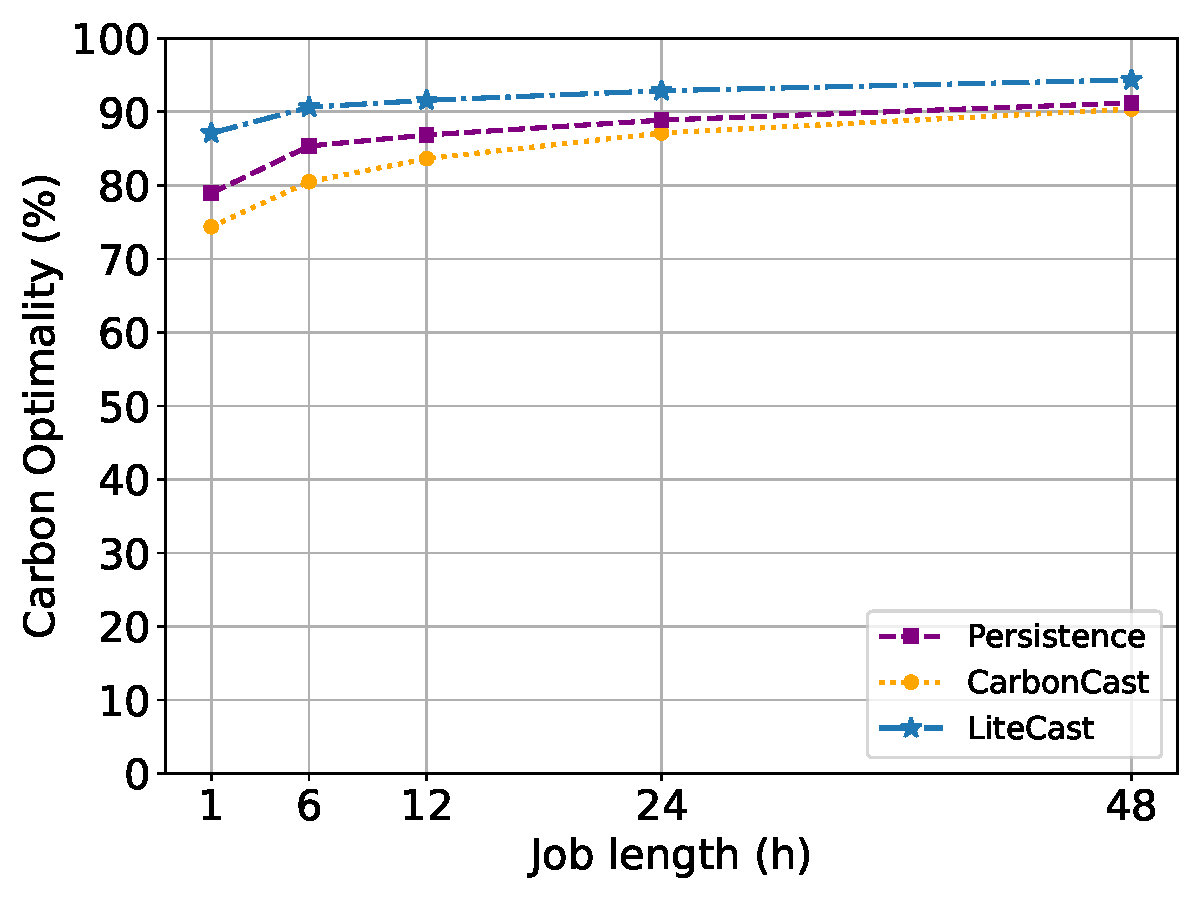
\includegraphics[width=\linewidth]{images/evaluation/fixed_slack/interruptable/Interruptable_Jobs_with_24_Hour_Slack_ensemble.pdf}
        \caption{$24$-hour slack}
        \label{fig:eval-interruptible-24h}
    \end{subfigure}
    \hfill
    \begin{subfigure}[t]{0.48\linewidth}
        \centering
        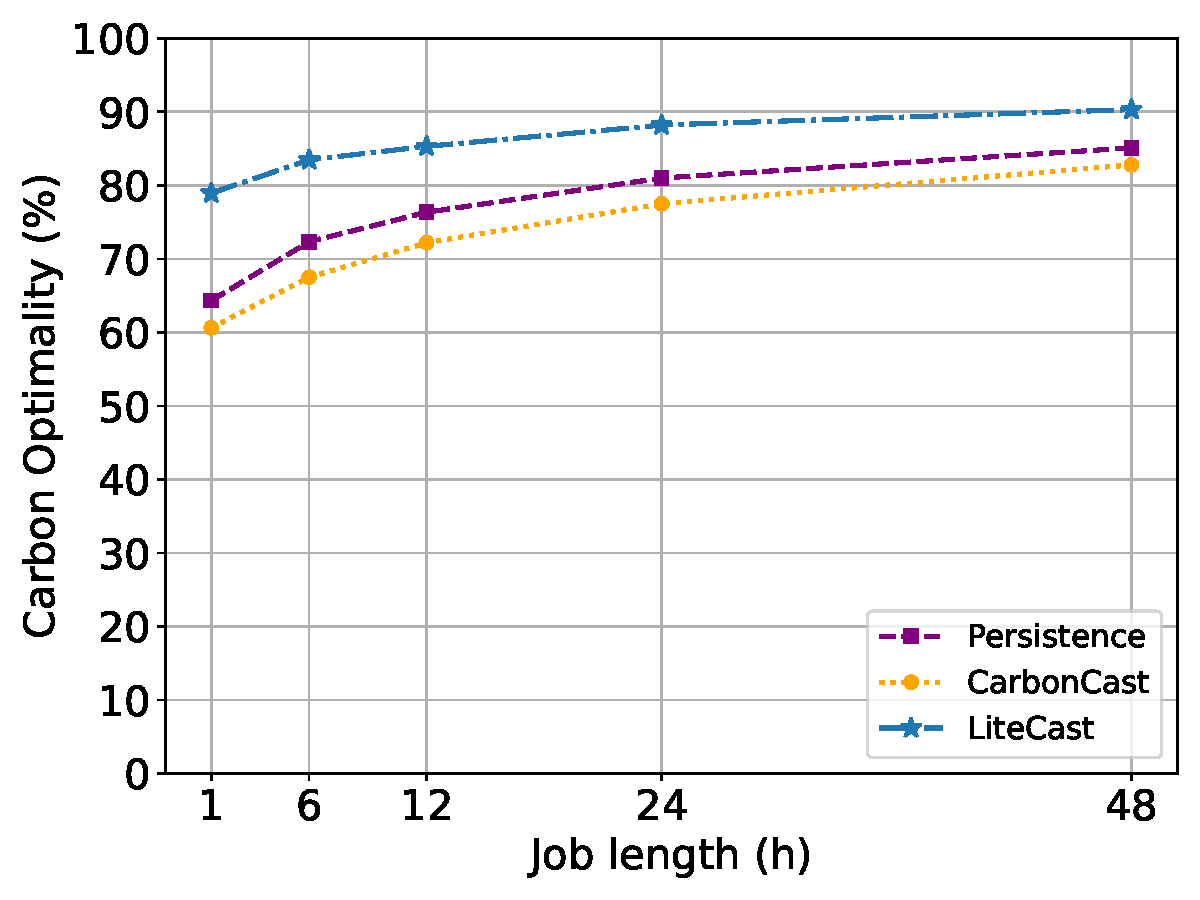
\includegraphics[width=\linewidth]{images/evaluation/fixed_slack/interruptable/Interruptable_Jobs_with_48_Hour_Slack_ensemble.pdf}
        \caption{$48$-hour slack}
        \label{fig:eval-interruptible-48h}
    \end{subfigure}

    \vspace{0.5em}

    \begin{subfigure}[t]{0.48\linewidth}
        \centering
        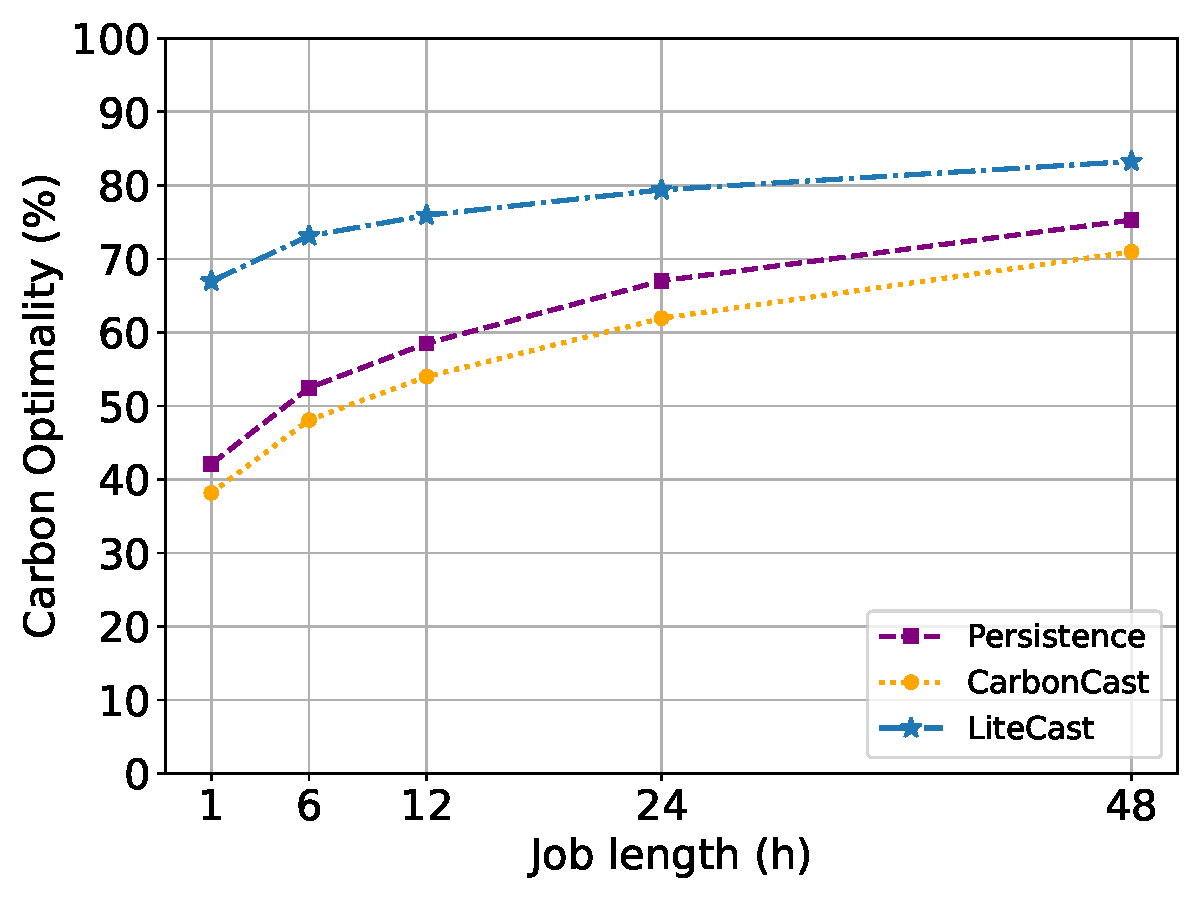
\includegraphics[width=\linewidth]{images/evaluation/fixed_slack/interruptable/Interruptable_Jobs_with_96_Hour_Slack_ensemble.pdf}
        \caption{$96$-hour slack}
        \label{fig:eval-interruptible-96h}
    \end{subfigure}
    \hfill
    \begin{subfigure}[t]{0.48\linewidth}
        \centering
        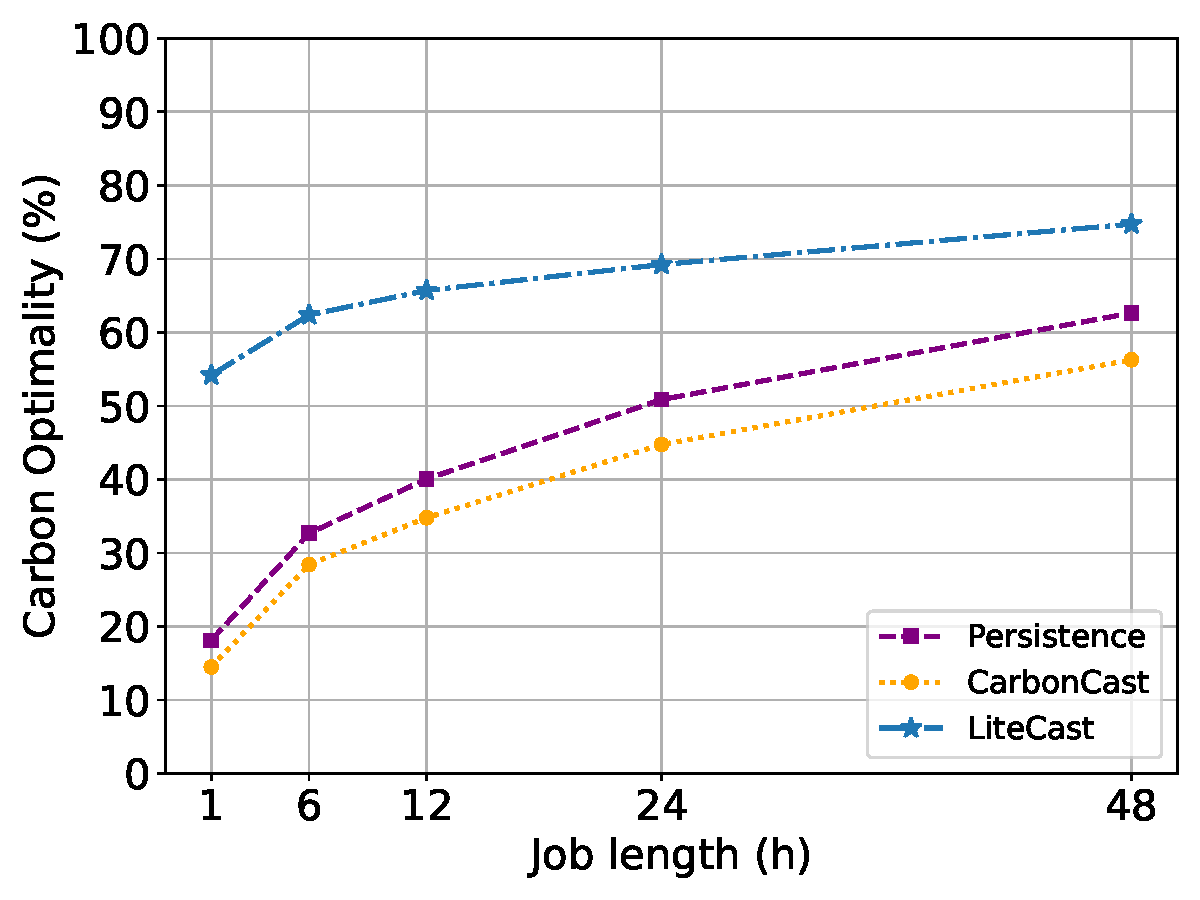
\includegraphics[width=\linewidth]{images/evaluation/fixed_slack/interruptable/Interruptable_Jobs_with_168_Hour_Slack_ensemble.pdf}
        \caption{$168$-hour slack}
        \label{fig:eval-interruptible-168h}
    \end{subfigure}
    \caption{Carbon optimality across all $48$ regions for interruptible jobs.}
    \label{fig:eval-carbon-optimality-interruptible}
\end{figure}

Figure~\ref{fig:eval-carbon-optimality-interruptible} reports the analogous results for interruptible jobs at the same four slack values.
LiteCast still outperforms CarbonCast, and the curves saturate at lower carbon optimality than in the continuous case.
Interruptible scheduling is fundamentally harder than continuous scheduling: rather than choosing a single start hour for a contiguous block, the scheduler must make $\mathcal{J}_{\text{length}}$ separate decisions about which individual hours have the lowest carbon intensity.
Each of those decisions is itself an ordering problem over the candidate window, so the forecast's rank-agreement with the realized signal is exercised $\mathcal{J}_{\text{length}}$ times rather than once.
Concordance therefore matters more for interruptible workloads than for continuous ones, because identifying the cleanest individual hours, especially the deepest troughs, depends entirely on the forecast preserving the correct ordering at those points.
A forecaster that misranks even a handful of the lowest-intensity hours loses optimality in proportion to how many of those hours the scheduler needs to fill.

% \subsection{Concordance Predicts Realized Savings}
% \label{sec:eval-temporal-concordance}

% % \begin{figure}[h]
% %     \centering
% %     \includegraphics[width=0.95\linewidth]{images/evaluation/concordance_vs_emissions.pdf}
% %     \caption{(a) Aggregate concordance index and additional emissions for LiteCast and CarbonCast across all regions and configurations. (b) Per-region additional emissions plotted against the grid's coefficient of variation (CV) of carbon intensity. Each marker is one region.}
% %     \label{fig:eval-concordance-vs-emissions}
% % \end{figure}

% Figure~\ref{fig:eval-concordance-vs-emissions} closes the loop between the forecast-quality results of \S\ref{sec:eval-forecast-quality} and the scheduling-outcome results above.
% Panel (a) aggregates concordance and additional emissions across all regions and configurations.
% LiteCast's roughly $15$-percentage-point concordance advantage over CarbonCast corresponds to an approximately twofold reduction in additional emissions: CarbonCast averages $36\%$ additional emissions over the oracle, LiteCast averages $22\%$, and LiteCast~+~Heuristic averages $17\%$.
% That a $15$-point concordance gain produces a $2\times$ swing in emissions is the operational restatement of the analytic point made in \S\ref{sec:method-concordance}: the scheduler depends on the forecast only through the ordering it induces, so improvements to ordering compound disproportionately in the realized objective.

% Panel (b) breaks the aggregate down per region, plotting each region's additional emissions against its coefficient of variation.
% Two features stand out.
% High-CV grids on the right side of the plot are harder for every forecaster, because their realized carbon intensity offers both the largest potential savings and the largest scope for ordering errors.
% Across the full CV range, LiteCast~+~Heuristic's scatter sits below CarbonCast's in $93\%$ of regions, with the biggest absolute gaps in the most variable grids --- precisely the grids where the concordance-versus-MAPE distinction in \S\ref{sec:eval-mape-vs-concordance} is sharpest.
% The few regions where CarbonCast is competitive are the lowest-CV grids in the bottom-left of the panel, where both forecasters are operating against a flat target and the choice of forecaster matters relatively little.
% This is the strongest aggregate evidence in the chapter for the central claim: \textit{the dimension of forecast quality that drives carbon savings is rank-preservation, not pointwise accuracy.}

\section{Spatial Carbon-Aware Scheduling}
\label{sec:eval-spatial}

Spatial scheduling is a second style of carbon-aware scheduling we test LiteCast on.
Instead of choosing \textit{when} to run a job within a single region, a spatial scheduler chooses \textit{where} to run it across multiple regions \cite{souza_casper_2023, gsteiger_caribou_2024}.
Spatial flexibility applies most naturally to cloud workloads such as web services, microservices, and AI inference, which can be moved between data centers with limited disruption.

\textbf{Experimental setup.}
Each spatial experiment is run between a pair of regions over a fixed $24$-hour window.
The window is divided into $\text{window}/\text{migrations}$ equal-length subdivisions; within each subdivision, the forecaster decides which of the two regions the job should be running in.
The oracle makes the same per-subdivision decisions using $f^{\text{act}}$, and we report carbon optimality as the ratio of the oracle's realized emissions to the forecaster's realized emissions.
We sweep this experiment across all pairs of grids in the $48$-region set, so every reported point is an aggregate over pairwise comparisons rather than a single region's behavior.
When the migration count equals $24$, the forecaster must choose the cleaner region on a per-hour basis, resulting in more chances to predict incorrectly.

\subsection{Overall Spatial Performance}
\label{sec:eval-spatial-overall}

\begin{figure}[!htbp]
    \centering
    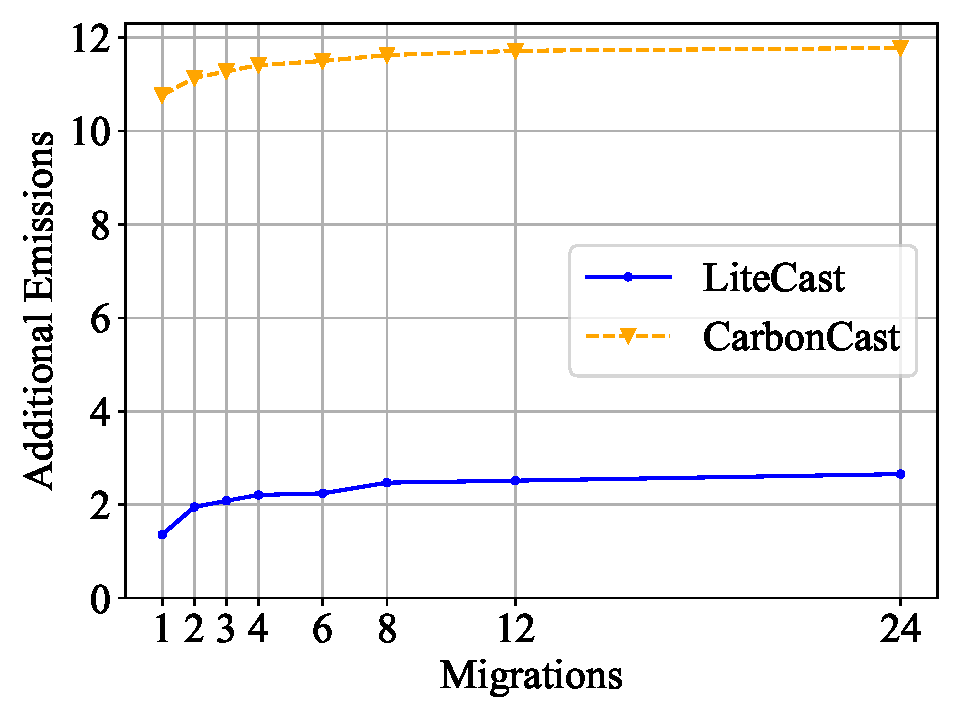
\includegraphics[width=0.95\linewidth]{images/evaluation/Comparing_CC_vs_LC_on_Spatial_Movement_Over_All_Grid_Pairs_for_a_24_hour_Slack_thesis.pdf}
    \caption{Spatial scheduling performance across all grid pairs at a $24$-hour slack.}
    \label{fig:eval-spatial-overall}
\end{figure}

Figure~\ref{fig:eval-spatial-overall} reports the aggregate carbon optimality of LiteCast and CarbonCast over all grid pairs at a $24$-hour slack.
The largest performance impact appears on grid pairs whose carbon intensities are similar: when the two regions are close, every per-subdivision decision turns on the forecaster correctly ordering them in that window, and small ranking errors translate directly into wrong-region choices.
On pairs where one region is consistently much cleaner than the other, both forecasters perform similarly because the cleaner region is easy to identify regardless of forecast precision.
LiteCast outperforms CarbonCast across the pair distribution by 9\%, and the gap is most pronounced on the similar-intensity pairs where the ordering question is hardest.

Spatial scheduling exercises the forecaster on a different kind of ordering question than the temporal case: rather than ranking hours within a single region, the forecaster must rank regions against each other within each subdivision of the window.
LiteCast's concordance advantage over CarbonCast carries over to this style of scheduling, with the largest gains appearing on grid pairs whose intensities are close enough that the cross-region ordering is non-trivial.
Spatial migration is more expensive to actually perform than temporal deferral, since the workload must be containerized, the data must be reachable from the destination region, and inter-region bandwidth has its own carbon cost, but those operational costs are orthogonal to the forecasting question that this chapter evaluates and we do not model them here.

% \subsection{Region Case Study: Denmark}
% \label{sec:eval-spatial-case}
%
% \begin{figure}[h]
%     \centering
%     \includegraphics[width=0.95\linewidth]{images/evaluation/spatial_case_denmark.pdf}
%     \caption{Spatial scheduling case study for a Denmark-originating job. The top panel shows the realized carbon intensity in Denmark, Germany, and the Netherlands over a one-week submission window; the bottom panel shows the execution region chosen at each scheduling decision by the oracle, LiteCast~+~Heuristic, and CarbonCast.}
%     \label{fig:eval-spatial-case-denmark}
% \end{figure}
%
% To illustrate the dynamics behind the aggregate numbers, Figure~\ref{fig:eval-spatial-case-denmark} examines a single region in detail.
% We pick Denmark as the home region for this case study because it is the region in our set where intra-day wind ramps are largest and where the spatial-versus-temporal tradeoff is therefore most active: in a low-wind Danish week, migrating to a neighboring grid can substantially reduce emissions, while in a high-wind Danish week Denmark itself is the cleanest available option.
% The figure overlays a week of realized carbon intensity for Denmark and two adjacent candidate regions (Germany and the Netherlands) and marks the execution region chosen at each decision point by the oracle, by LiteCast~+~Heuristic, and by CarbonCast.
%
% The qualitative pattern parallels the within-region case in \S\ref{sec:eval-temporal-samples}.
% When Denmark and a neighbor have similarly low forecasted intensities, LiteCast may diverge from the oracle on the choice of region without materially diverging on realized emissions, because the cross-region ordering at the chosen window is preserved.
% The decisions where the heuristic's refit step matters most are the wind-ramp transitions: in the hour before Denmark's wind output collapses, the heuristic's pseudo-oracle picks up the regime shift from in-flight observations and migrates the job to Germany before the static forecast has had a chance to react.
% These transition-hour decisions account for a disproportionate share of the spatial heuristic's lead over LiteCast without the heuristic.

\section{Cluster Workload Trace}
\label{sec:eval-cluster}

The preceding sections evaluate isolated jobs at controlled lengths and slacks.
A practical scheduler must handle a heterogeneous mix of jobs whose lengths and slacks are dictated by users rather than by the experimenter, and whose statistical distribution may differ substantially from the uniform sweep we have used so far.
We test this by replaying the KIT workload trace \cite{kit_trace} from the Parallel Workloads Archive, which records eighteen months of accounting data from the ForHLR~II supercomputer at the Karlsruhe Institute of Technology.

\subsection{Trace and Replay Setup}
\label{sec:eval-cluster-trace}

The KIT trace contains roughly $114{,}000$ jobs submitted by real cluster users between 2016 and 2018, but was cut to half a year due to computation and data limitations.
Job lengths span four orders of magnitude, from sub-minute jobs to multi-day jobs, with a heavy tail of short jobs typical of supercomputing workloads.
We replay the trace by treating each recorded submission as an arrival into a carbon-aware scheduler and setting each job's slack equal to its observed waiting time in the trace, so the replay preserves both the length distribution and the slack distribution from real user behavior rather than imposing a synthetic sweep.
Because LiteCast operates at hourly granularity, we round each job's length and slack to the nearest hour before scheduling.
In addition, since the trace did not provide any slack length for the jobs, we added 2 times the job length for the slack. 
This allows enough space for the forecasters to make a meaningful scheduling decision.
The replay is run independently in each of the $48$ regions, allowing us to report per-region savings as well as aggregate savings.

\subsection{Per-Region Savings}
\label{sec:eval-cluster-savings}

\begin{figure}[!htbp]
    \centering
    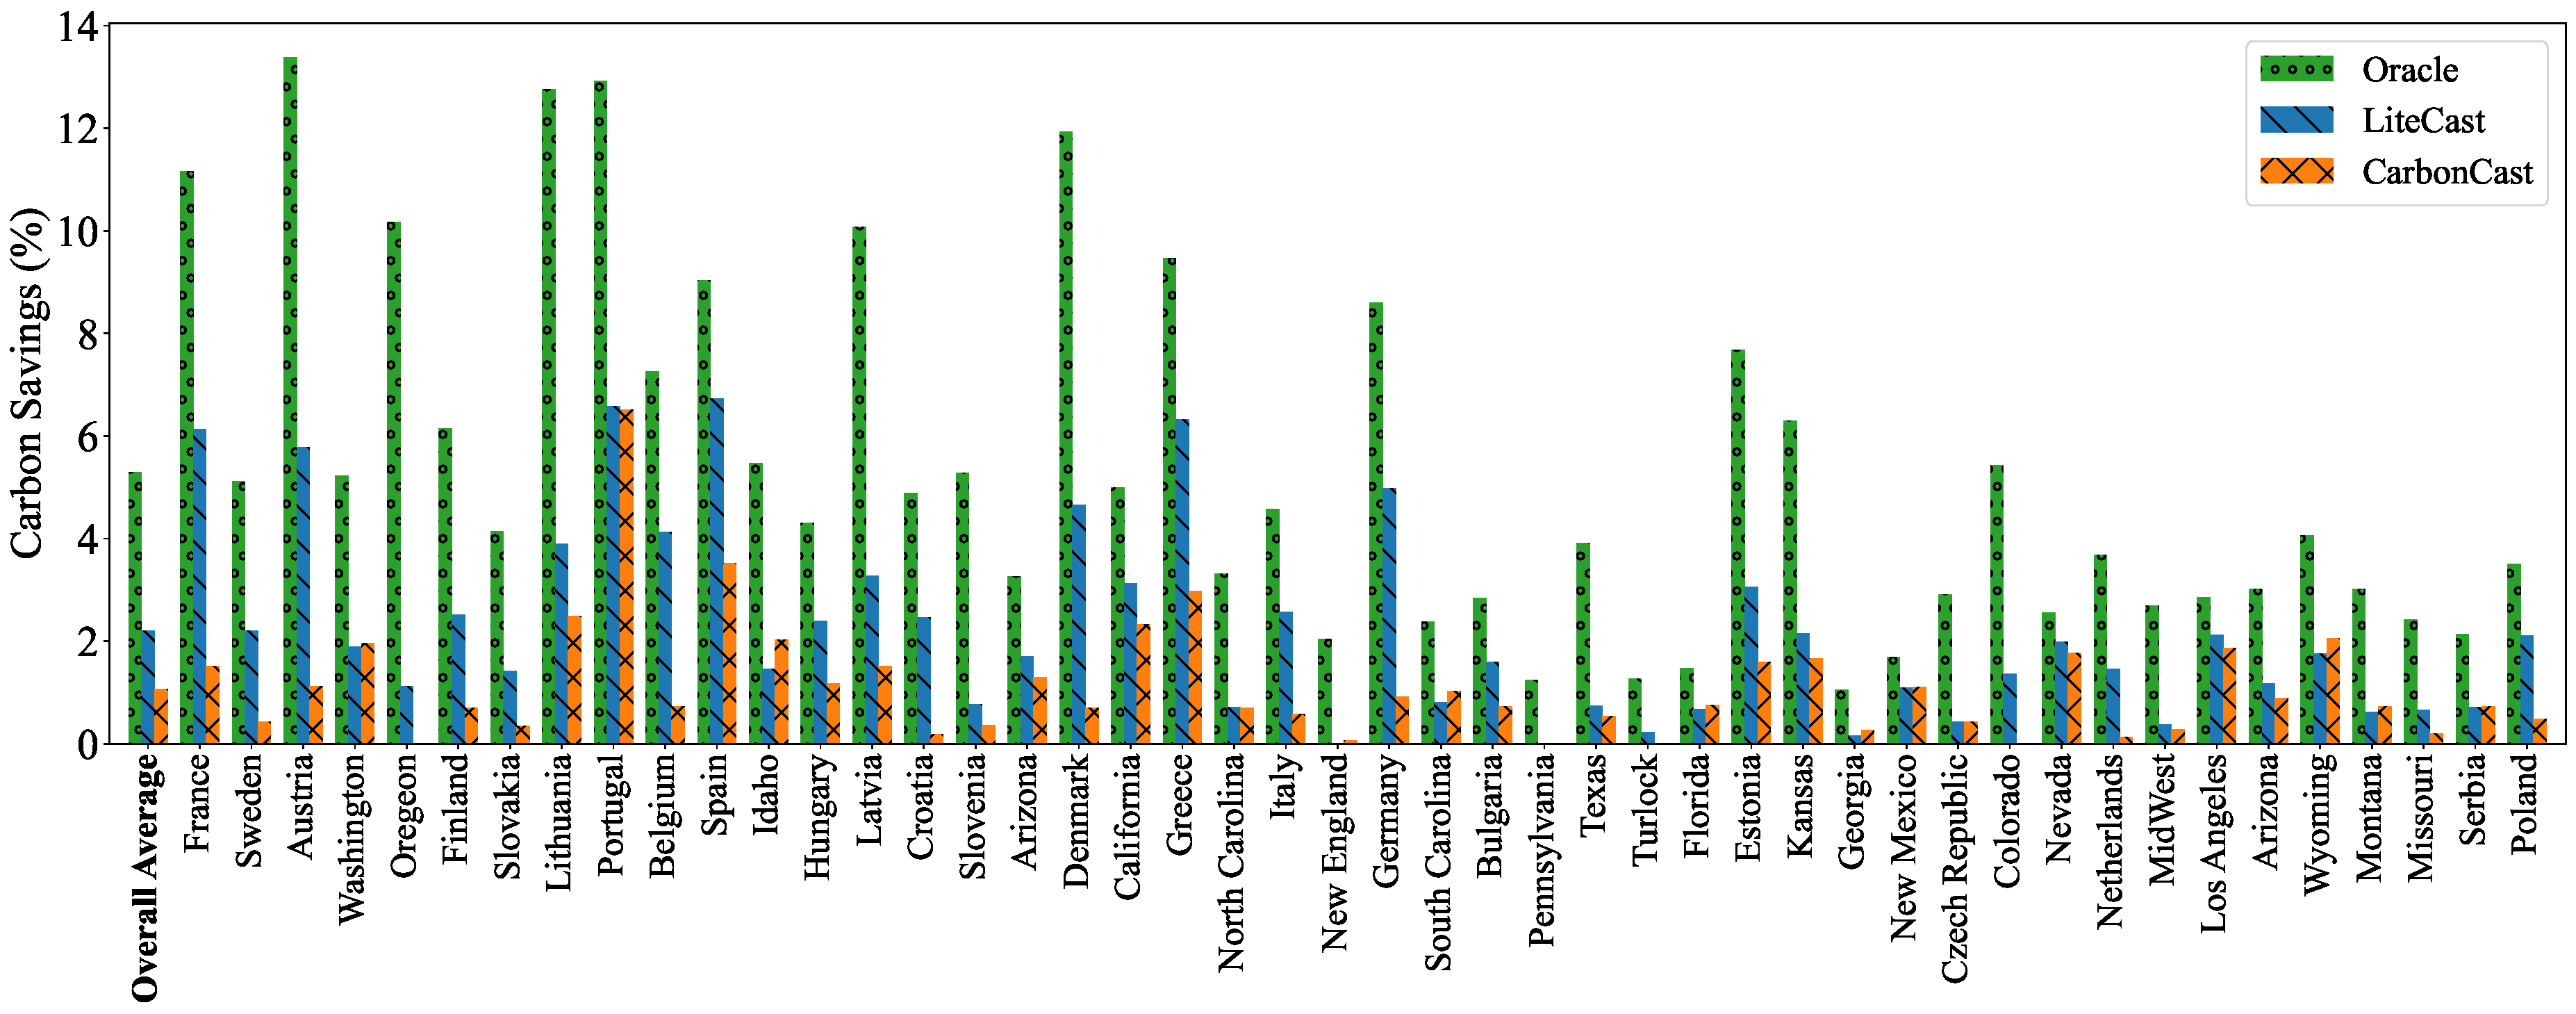
\includegraphics[width=0.95\linewidth]{images/evaluation/workload_plot_thesis.pdf}
    \caption{Per-region carbon savings on the KIT trace replay across $48$ regions. The leftmost cluster shows the cross-region average.}
    \label{fig:eval-kit-trace}
\end{figure}

Figure~\ref{fig:eval-kit-trace} reports per-region carbon savings for the trace replay.
LiteCast delivers an average savings of $2\%$ over a carbon-blind FIFO baseline and trails the oracle by approximately $3.5$ percentage points on average.
It outperforms CarbonCast in $74\%$ of the $48$ regions; the regions where CarbonCast is competitive are the low-CV grids in which absolute savings are small for every forecaster.
The trace is dominated by short jobs, as roughly $80\%$ of jobs run for less than an hour, which structurally limits the absolute scope for carbon-aware optimization: a one-hour job with a two-hour slack has only a handful of candidate start hours, regardless of the forecaster's quality.

\subsection{Implications}
\label{sec:eval-cluster-discussion}

The KIT result demonstrates that the chapter's central finding survives the messy reality of a real cluster workload mix.
LiteCast's concordance-driven advantage is robust to the heavy short-job tail of the trace, recovering meaningful savings that CarbonCast leaves on the table even when the average savings ceiling is low.
The numbers are smaller in absolute terms than the synthetic sweep of \S\ref{sec:eval-temporal} because the KIT job-length distribution does not include a significant portion of large-scale jobs.
The relative ordering among policies, however, is unchanged.

\section{Discussion}
\label{sec:eval-discussion}

The results above support the chapter's framing question with two empirical claims and a set of caveats.

\subsection{Concordance, not Precision, Drives Realized Savings}
\label{sec:eval-discussion-concordance}

The standalone forecast-quality comparison in \S\ref{sec:eval-forecast-quality} shows that LiteCast achieves consistently higher concordance.
The carbon-optimality results in Figures~\ref{fig:eval-carbon-optimality-continuous},~\ref{fig:eval-carbon-optimality-interruptible}, and~\ref{fig:eval-spatial-overall} track concordance, not MAPE.
% The per-region scatter in Figure~\ref{fig:eval-concordance-vs-emissions}(b) makes the relationship explicit: the regions where LiteCast's concordance advantage is largest are also the regions where its emissions advantage is largest.
This is the structural relationship predicted by the analysis in \S\ref{sec:method-concordance}: the scheduler depends on the forecast only through the ordering it induces, so ordering is what should be optimized.
The contribution of this thesis is to demonstrate, with $48$ regions and the workload sweeps above, that concordance is a significant factor in making significant carbon-optimal scheduling decisions.

\subsection{Lightweight Statistical Models Can Match Heavyweight Neural Models}
\label{sec:eval-discussion-lightweight}

SARIMAX, trained on a month-long rolling window of hourly data, outperforms CarbonCast, a deep machine learning model trained on a year of history.
The standard intuition that more data and more parameters give more accurate forecasts does not transfer to carbon-aware scheduling, because the relevant signal is not accuracy but rank-preservation, and a model with a small, recent training window can capture local diurnal and weather-driven ordering structure as well as or better than a model trained on long histories that necessarily averages across regime shifts.

This has two practical implications.
% First, LiteCast is deployable in regions with limited historical data, which includes most of the developing-world grids where carbon-aware scheduling has the largest potential impact and where multi-year hourly histories are not always available.
First, LiteCast is deployable in regions with limited historical data, which makes data collection more practical.
% Second, the low retraining cost is what makes the adaptive heuristic of \S\ref{sec:method-heuristic} feasible at the cadence at which it operates: refitting a SARIMAX model on hourly observations as a job waits costs seconds on a CPU, whereas refitting a deep ensemble at the same cadence would require dedicated GPU infrastructure and would force the scheduler to choose between adaptivity and operating cost.
Second, the low training cost makes the SARIMAX model practical to train on common hardware and allows the model to be more reactive to the changes in the carbon intensity. 
LiteCast's gains in Figures~\ref{fig:eval-carbon-optimality-continuous} and~\ref{fig:eval-carbon-optimality-interruptible} are conditional on the lightweight base model.

% \subsection{Limitations}
% \label{sec:eval-discussion-limitations}

% Three caveats are worth noting.
% First, SARIMAX produces deterministic point forecasts, which makes concordance well-defined but discards any signal about forecast uncertainty.
% Workloads whose scheduling decisions depend on calibrated probabilities --- for example, online competitive algorithms with risk-adjusted objectives \cite{lechowicz_learning_2025} or systems that must respect explicit confidence intervals --- are not directly served by this design.
% Second, the evaluation uses average carbon intensity, following the GHG protocol's Scope~2 convention and the prior carbon-aware scheduling literature; results on marginal-intensity signals may differ \cite{sukprasert_limitations_2024}, especially in regions whose marginal generator profile diverges substantially from the demand-weighted average.
% Third, the evaluation covers $48$ regions in the USA and Europe; grids elsewhere with substantially different generation mixes, weather regimes, or operational patterns may require validation before deployment.
% None of these limitations affect the chapter's central claim --- that rank-preservation is the relevant forecast quality for carbon-aware scheduling --- but they bound the regimes in which the specific LiteCast realization is the right tool.
